%\chapter*{Introduction}
\chapter{Introduction}
%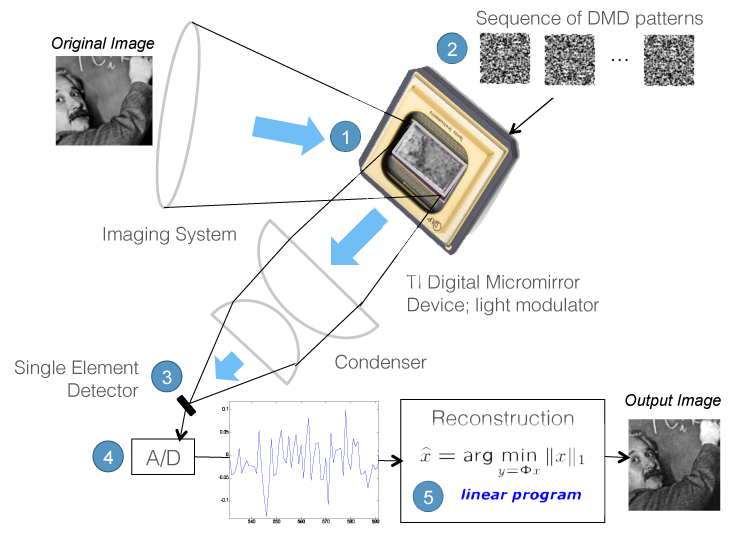
\includegraphics{Img1.png}
%\addcontentsline{toc}{chapter}{Introduction}
Compressed sensing (CS) is a novel technique based on the discoveries done by Candes et al. \cite{CandesR07} and Donoho \cite{Donoho01}. They showed that as long as certain conditions are met, a signal can be fully recoverd from a small number of measurements. Due to this fact, CS is suitable for many Signal Processing (SP) applications and specifically image processing. An example of this is the publication made by Duearte et al. \cite{duarte2008single}. In their work they  proposed an imaging sensor capable of sampling and compressing the signal at the same time. Image number 1 shows the general path for CS in pothography applications. Such a sensor can be energy efficient since the measurements taken are much less that those made by normal sensors and there is no compression face after the measuremnts are taken. As a result, the indutry and the research community have been very interested and have actively done research during the last years in order to designed a sensor capable of giving both better energy afficience and as well as good algorithms capable of yielding high quality for the recovered-images. Unfortunately, everything comes with a cost and recovering an original image from compressed measurents is a problem that has high complexity and computacionally expensive to solve. This problems are commonly referred to as inverse problems since one tries to recover a signal from under-sampled measurements. \

Many Algorithms have been proposed for reconstruction, among the most widely known and recognize one can find \cite{metzler2014denoising,dong2014compressive, li2013efficient,mun2009block,chen2011compressed,fowler2011multiscale}. Nevertheless, most of them suffer from the same disadavnatages because they follow the most general approach for the reconstruction process. First, they solve an optimization problem which implies the use of iterations until a possible solution is obtained. Because of that most those algorithms are called iterative. Second,   


        

